%!TEX program = xelatex
%!TEX TS-program = xelatex
%!TEX encoding = UTF-8 Unicode

\documentclass[12pt,UTF8]{ctexart}
\usepackage{graphicx}
\usepackage{geometry}
\usepackage{multicol}
\usepackage{indentfirst}
\setlength{\parindent}{2em}
\usepackage{pgfplots}
\usepackage{cite}
\setlength{\parindent}{2em}
\usepackage{amsmath}
\usepackage[ruled,linesnumbered]{algorithm2e}
\usepackage{amssymb}
\usepackage{enumerate}
\usepackage{fontspec,xltxtra,xunicode}
\XeTeXlinebreakskip = 0pt plus 1pt minus 0.1pt
\renewcommand{\baselinestretch}{1.5}
%\usepackage[all]{background}
%\usepackage{wallpaper}
%\usepackage{tikz} %加水印用
%\usepackage{eso-pic}
% \setromanfont{Songti SC}
\defaultfontfeatures{Mapping=tex-text}
\XeTeXlinebreaklocale “zh”
\usepackage{subfigure}
\usepackage{titling,setspace}
\usepackage{enumerate}
\usepackage{amsmath,amssymb,amsfonts}
\usepackage{listings}
\lstset{language=C++}%这条命令可以让LaTeX排版时将C++键字突出显示
\lstset{breaklines}%这条命令可以让LaTeX自动将长的代码行换行排版
\lstset{extendedchars=false}%这一条命令可以解决代码跨页时,章节标题,页眉等汉字不显示的问题
\lstset{                     
  	language=[ANSI]{C},
  	backgroundcolor=\color{white},
	basicstyle=\footnotesize,
	breakatwhitespace=false,
	breaklines=true,
	captionpos=b,
	commentstyle=\color{gray},
	directivestyle=\color{blue},
	extendedchars=false,
	frame=single,%shadowbox
	framerule=0pt,
	keywordstyle=\color{blue}\bfseries,
  	morekeywords={*,define,*,include...},
  	numbersep=5pt,
  	rulesepcolor=\color{red!20!green!20!blue!20},
  	showspaces=false,
  	showstringspaces=false,
 	showtabs=false,
  	stepnumber=2,
  	stringstyle=\color{purple},
  	tabsize=4,
  	title=\lstname
}
\usepackage{comment}
\usepackage{float}
\usepackage{multicol,multirow}
\usepackage[unicode=true,%本行非常重要 支持中文目录hyperref CJKbookmarks对二级目录没用
	colorlinks,
	linkcolor=black,
	anchorcolor=black,
	citecolor=black,
	CJKbookmarks=false]{hyperref}
\usepackage{xcolor}
\geometry{top=25mm,bottom=25mm,left=25mm,right=25mm}
\pagestyle{plain}%删除页眉
\renewcommand\maketitlehooka{\null\mbox{}\vfill} % 标题页
\renewcommand\maketitlehookd{\vfill\null}
\renewcommand\tablename{表}
\renewcommand{\figurename}{图}
\def\equationautorefname{式}%
\def\footnoteautorefname{脚注}%
\def\itemautorefname{项}%
\def\figureautorefname{图}%
\def\tableautorefname{表}%
\def\partautorefname{篇}%
\def\appendixautorefname{附录}%
\def\chapterautorefname{章}%
\def\sectionautorefname{节}%
\def\subsectionautorefname{小小节}%
\def\subsubsectionautorefname{subsubsection}%
\def\paragraphautorefname{段落}%
\def\subparagraphautorefname{子段落}%
\def\FancyVerbLineautorefname{行}%
\def\theoremautorefname{定理}%
% \lstset{language=c++,basicstyle=\small,escapechar=`}
\setlength{\droptitle}{-100pt}%减少标题与页眉距离
\title{{\Huge Project 1\\火车调度}}
\usepackage{cleveref}
\vspace{100pt}
\renewcommand\contentsname{目录}
\author{\vspace{200pt}\quad\\
计科一班 17341009 曾天宇\\
计科一班 17341015 陈鸿峥\\
计科二班 17341059 黄杨峻}
\date{}

\begin{document}

\clearpage\maketitle
\thispagestyle{empty}

\newpage
\tableofcontents
\setcounter{page}{1}

\section{题目要求}
给定一个任意的车厢排列次序,设计一个软件系统调度排列车厢,使其按照从1到n的次序输出。要求给出调度详细步骤,并统计出所用栈个数及调度总步数。

\section{数据结构与算法}
首先这道题是一个典型问题——栈排序的改编,本质来说,题目中给到的缓冲轨道就是用于排序的辅助栈,由于序列不同需要到的辅助栈数目亦不同。考虑到经济因素,我们认为用最少的缓冲轨道实现车厢重排的算法为最优。

本次实验我们小组设计了两种不同的算法,具体如下。

方法一我们使用的是模拟的方法,这个方法实现的方法分为两个部分,分别为出站部分与进轨部分。我们假设当前应当驶出车站的火车车厢编号为$\text{now}$,缓冲轨道分别为$\text{station}[i],i\in\{0,1,2,\ldots\}$。出栈判断的对象是当前火车队头以及多个缓冲轨道的栈顶,首先判断队头的火车是否能直接出站,若不能,则考虑栈顶的每个车厢是否能够出栈,重复这个过程直到队头或者栈顶车厢无法出栈为止。随后我们开始进轨判断的部分:遍历所有已经使用的栈,寻找第一个可以插入此车厢的栈进行push操作,若无栈满足要求,则使用新的栈参与调度。满足push条件的栈条件如下:若栈顶元素大于车厢编号,则允许插入,若栈顶车厢编号小于车厢编号,则不允许,证明:

若栈顶车厢编号小于车厢编号($\text{stack}[i].\text{top}()<\text{train}$),由栈性质可知,当编号大的车厢处于栈顶时,位于该车厢下的车厢无法出栈,但位于下方的车厢编号更小,若不先出栈,顶部的车厢也无法出栈,故出入栈应满足上述条件。

方法二是建立在对数列的增减性的分析上,我们在反向读入数据的时候能够分析需要调整序列的变化情况。与方法一类似的有:如果遇到即将能够出栈的直接出栈;如果不能直接出栈的,则要判断增减性和是否有栈,如果没有栈在内存则创建新栈;如果存在栈在内存,且当前的变化为递减序列,则创建新的栈存放数据;如果存在栈在内存,且当前的变化为递增序列,则查找栈顶部数据离目标数最近的一个栈进行存放。这样利用类似于贪心的策略,能够有效减少栈的使用。

\newpage
\section{测试数据、结果及分析}
% (所输入的数据及相应的运行结果,运行结果要有提示信息,运行结果采用截图方式给出。)

测试数据为\autoref{tab:data} .

\begin{table}[H]
	\caption{测试数据表}
	\label{tab:data}
	\centering
	\begin{tabular}{|c|c|c|}
	\hline
	组别 & 车厢数目 & 车厢顺序\\
	\hline
	1 & 9 & 7 6 8 9 5 3 4 2 1 \\
	2 & 8 & 1 8 7 6 5 4 3 2 \\
	3 & 10 & 8 7 9 10 6 4 5 2 3 1 \\
	4 & 9 & 1 2 3 4 5 6 7 8 9\\
	\hline	
	\end{tabular}
\end{table}

下面是我们两种方法的运行结果:

方法一:
\begin{figure}[H]
\caption{方法一的运行结果}
\label{fig:method1}
\centering
\begin{tabular}{cc}
	\subfigure{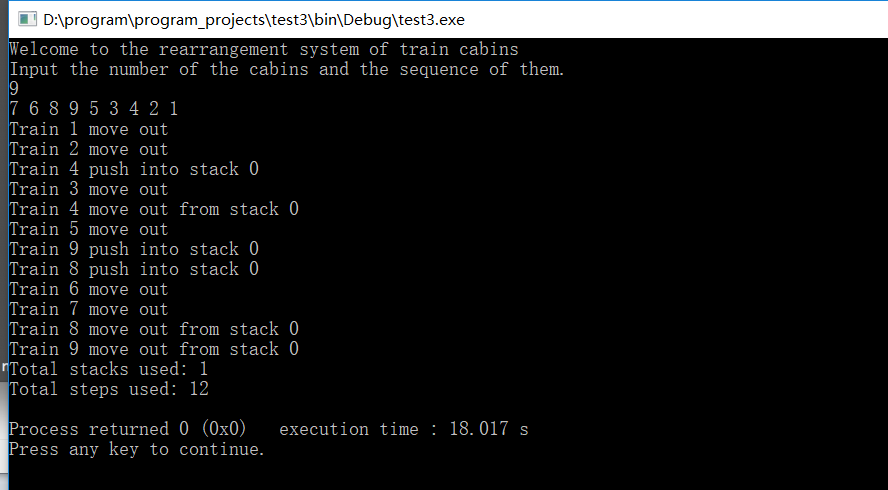
\includegraphics[width = 220pt]{Pics/pic3}}	&
	\subfigure{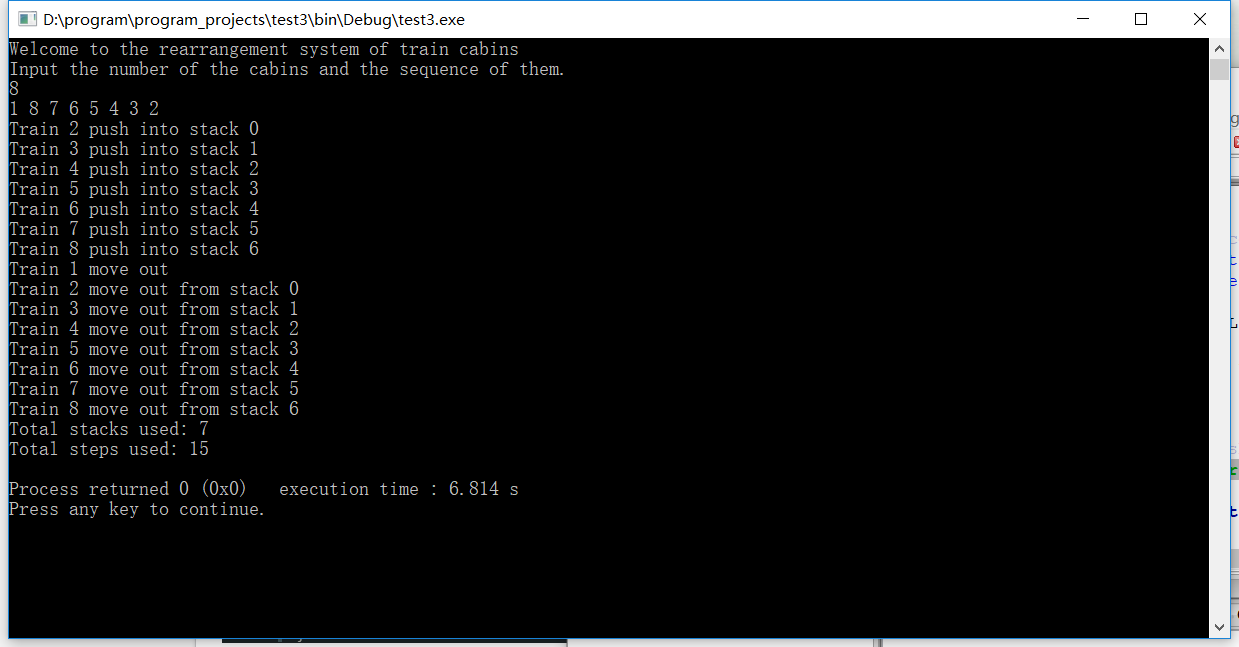
\includegraphics[width = 220pt]{Pics/pic4}}\\
	\subfigure{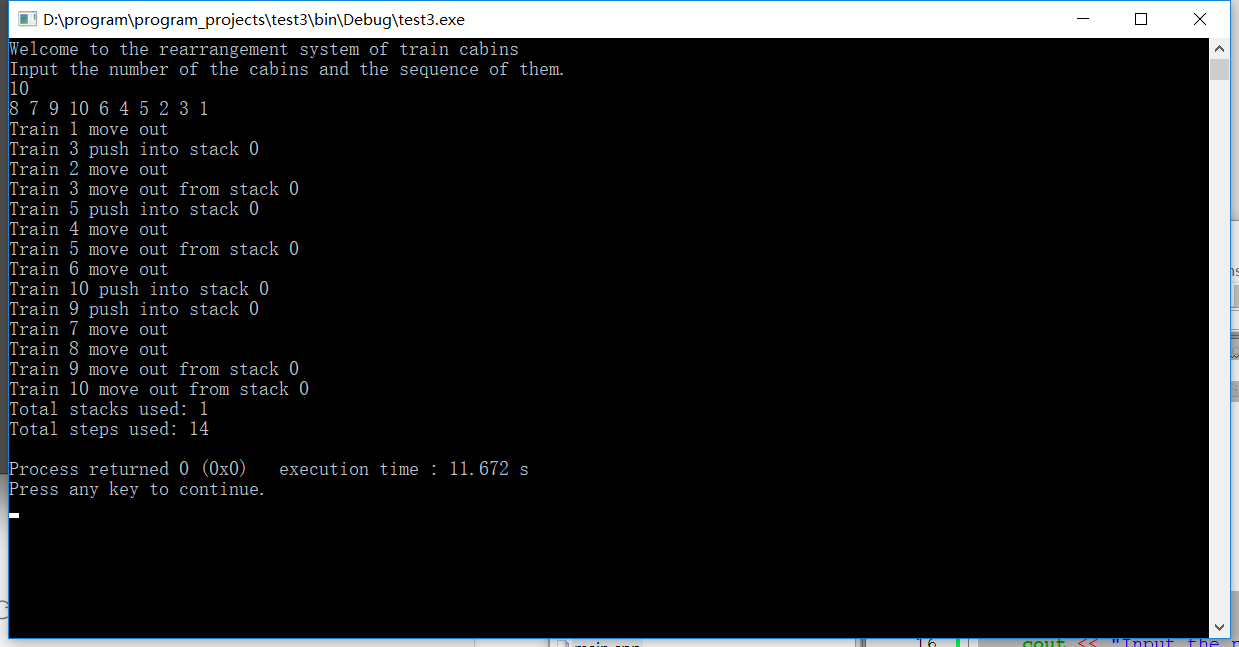
\includegraphics[width = 220pt]{Pics/pic6}}	
&	\subfigure{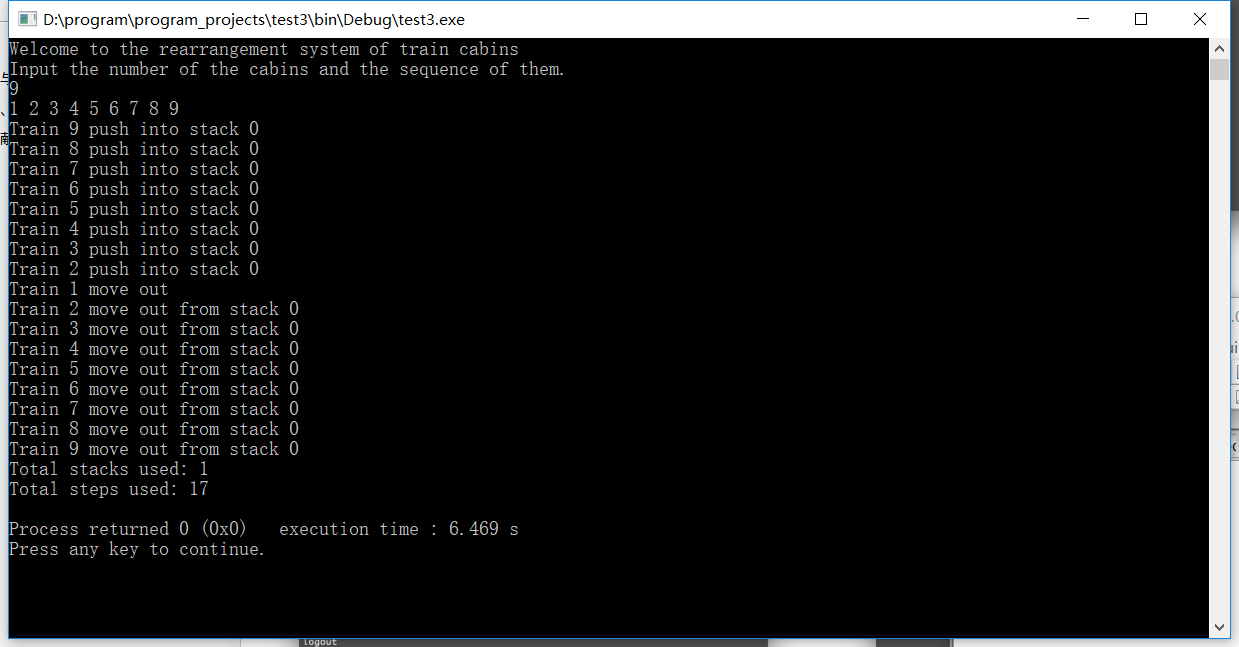
\includegraphics[width = 220pt]{Pics/pic8}}	\\
\end{tabular}
\end{figure}

\newpage
方法二:

\begin{figure}[H]
\caption{方法二的运行结果}
\label{fig:method2}
\centering
\begin{tabular}{cc}
	\subfigure{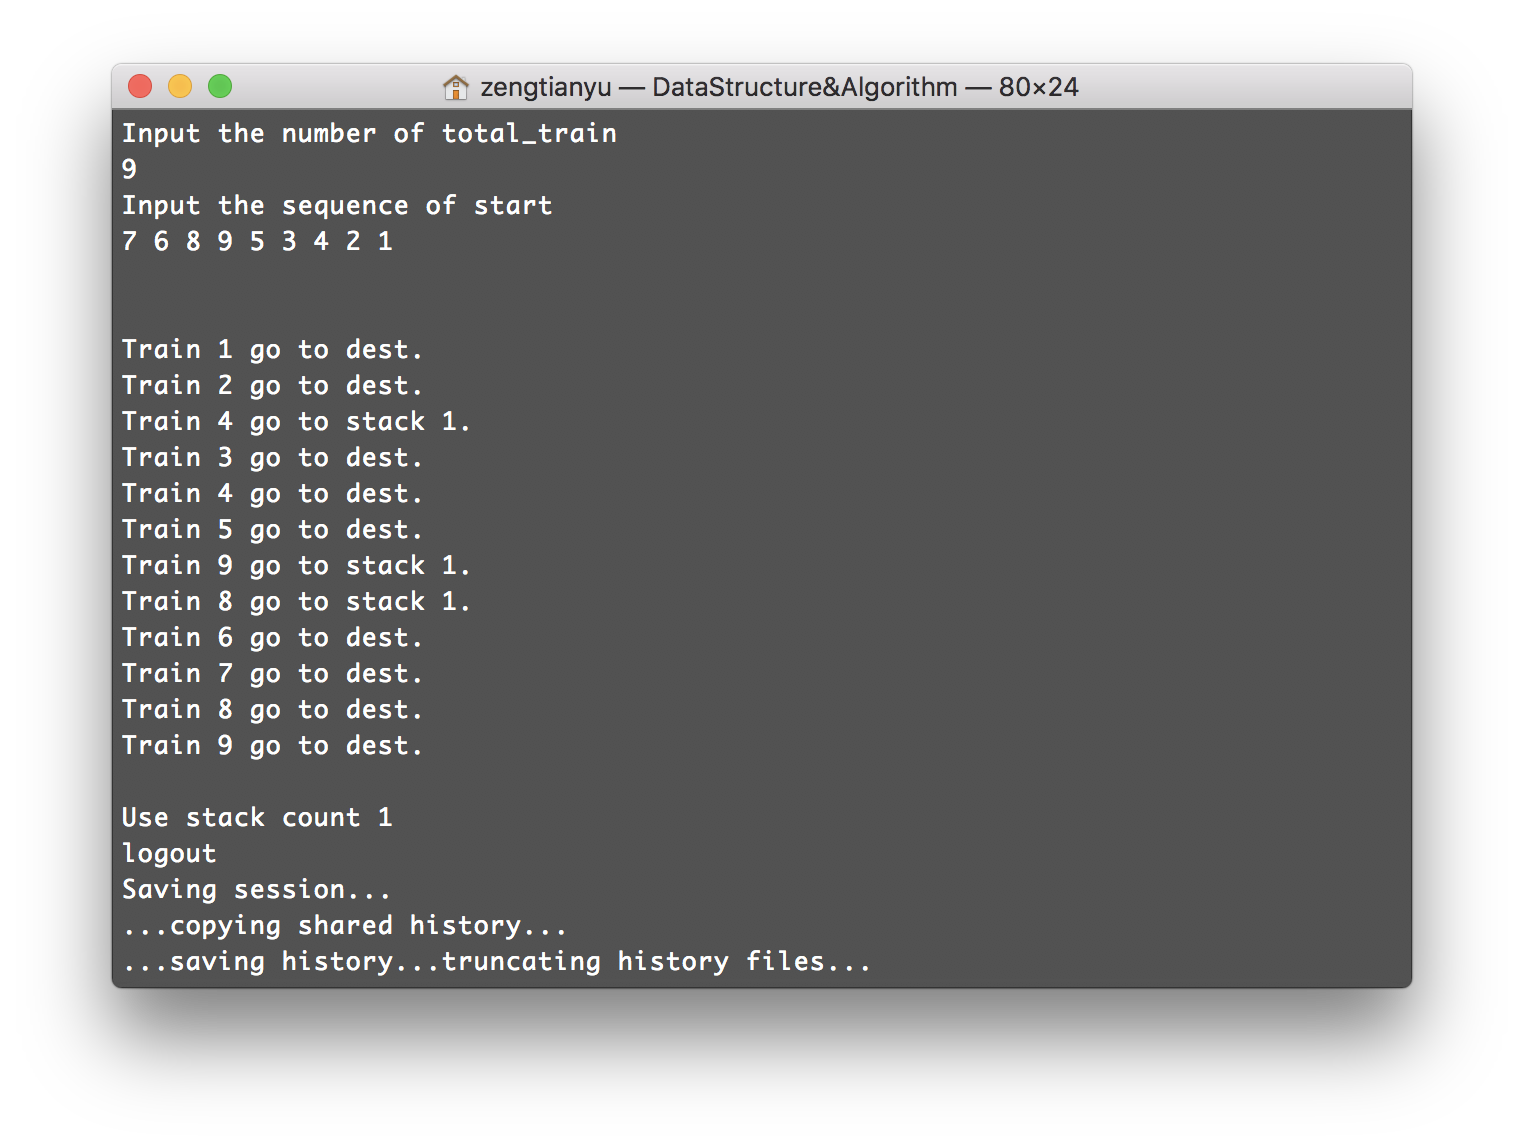
\includegraphics[width = 220pt]{Pics/pic1}}	&
	\subfigure{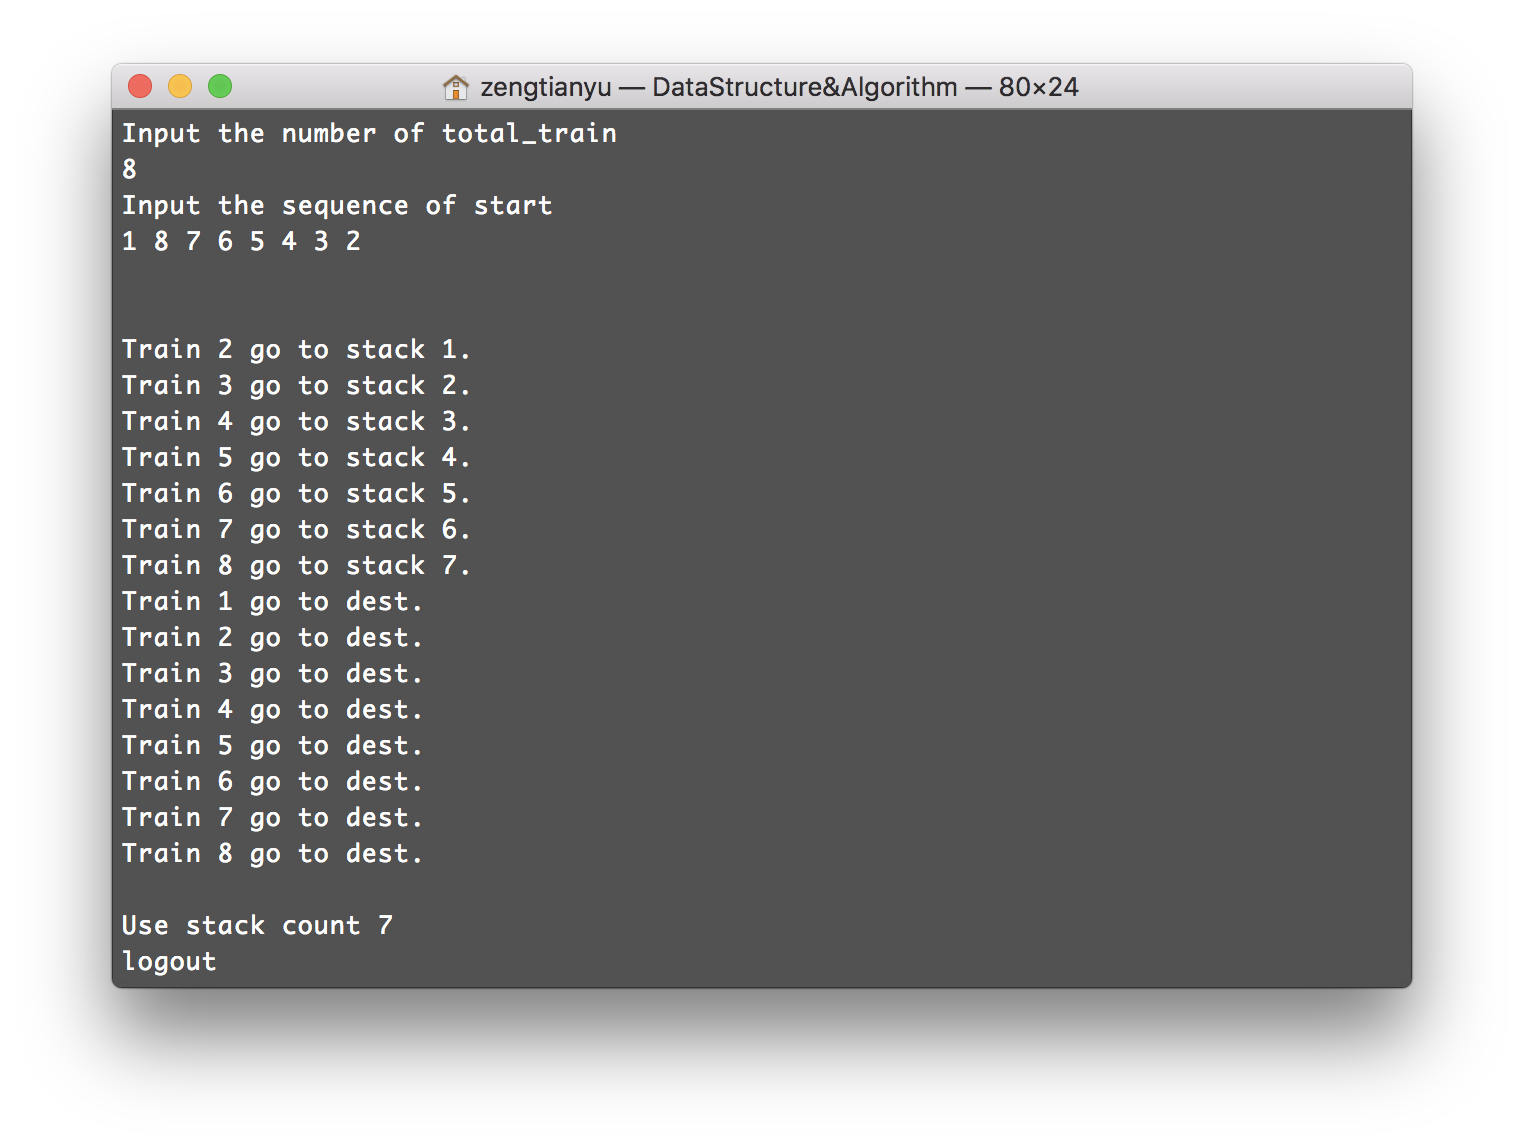
\includegraphics[width = 220pt]{Pics/pic2}}\\
	\subfigure{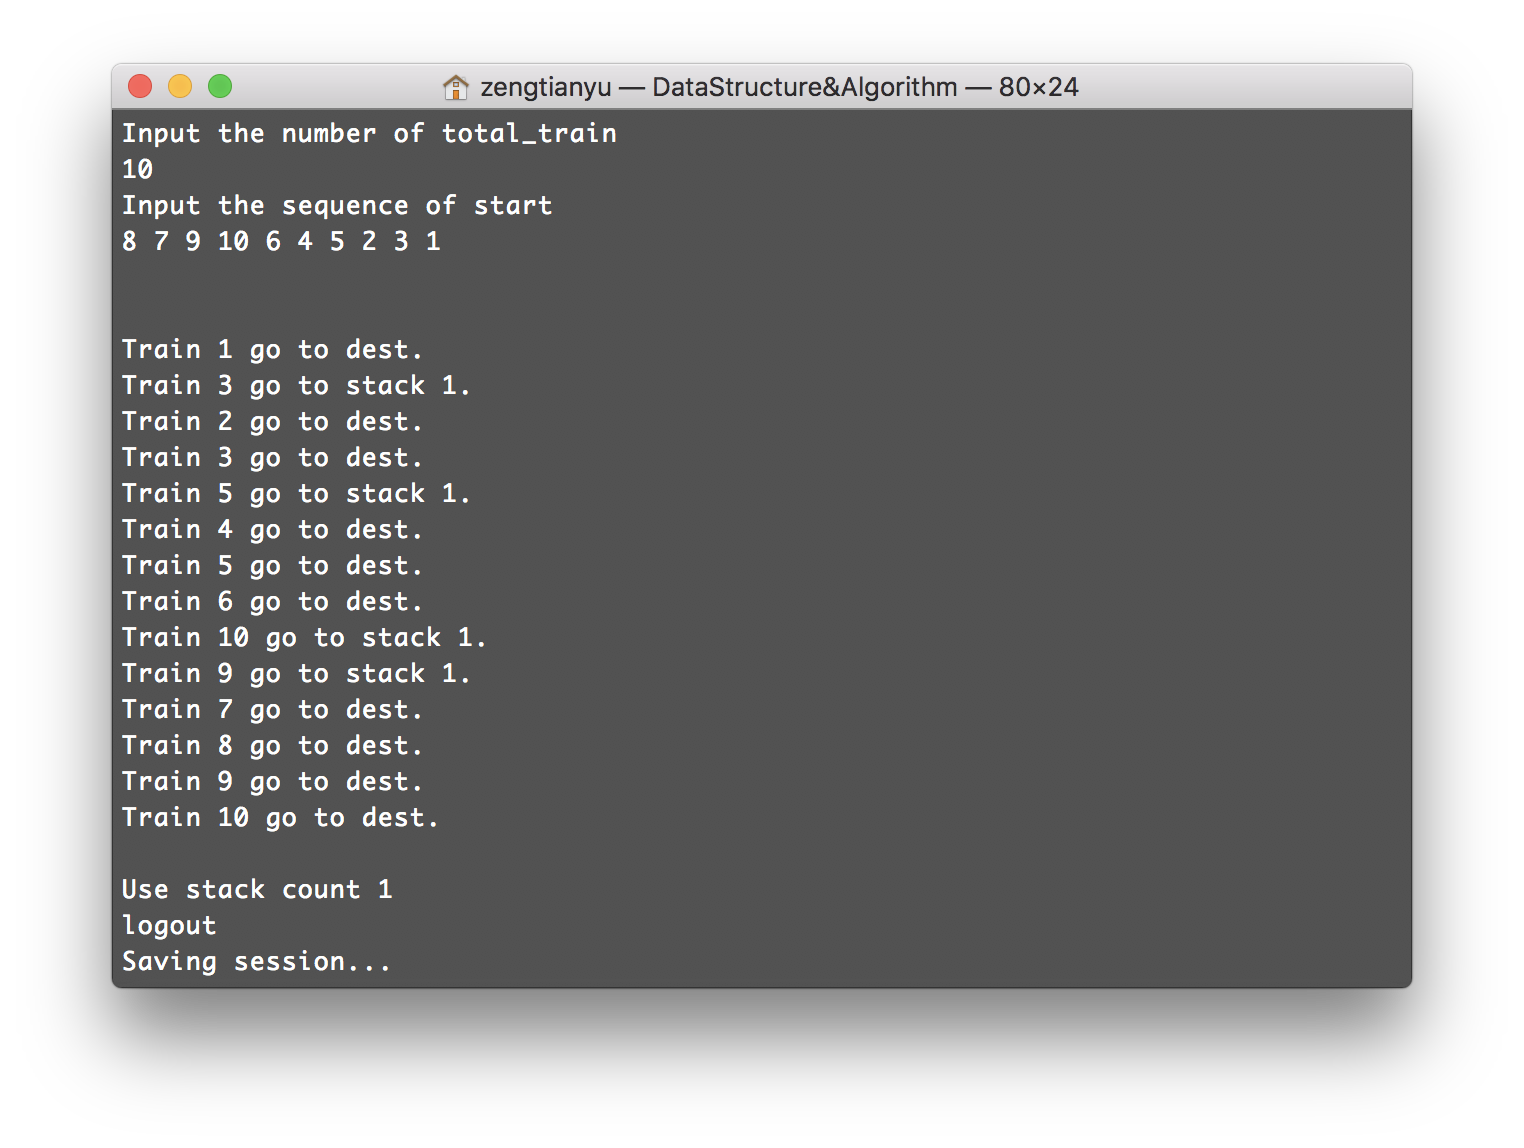
\includegraphics[width = 220pt]{Pics/pic5}}	
&	\subfigure{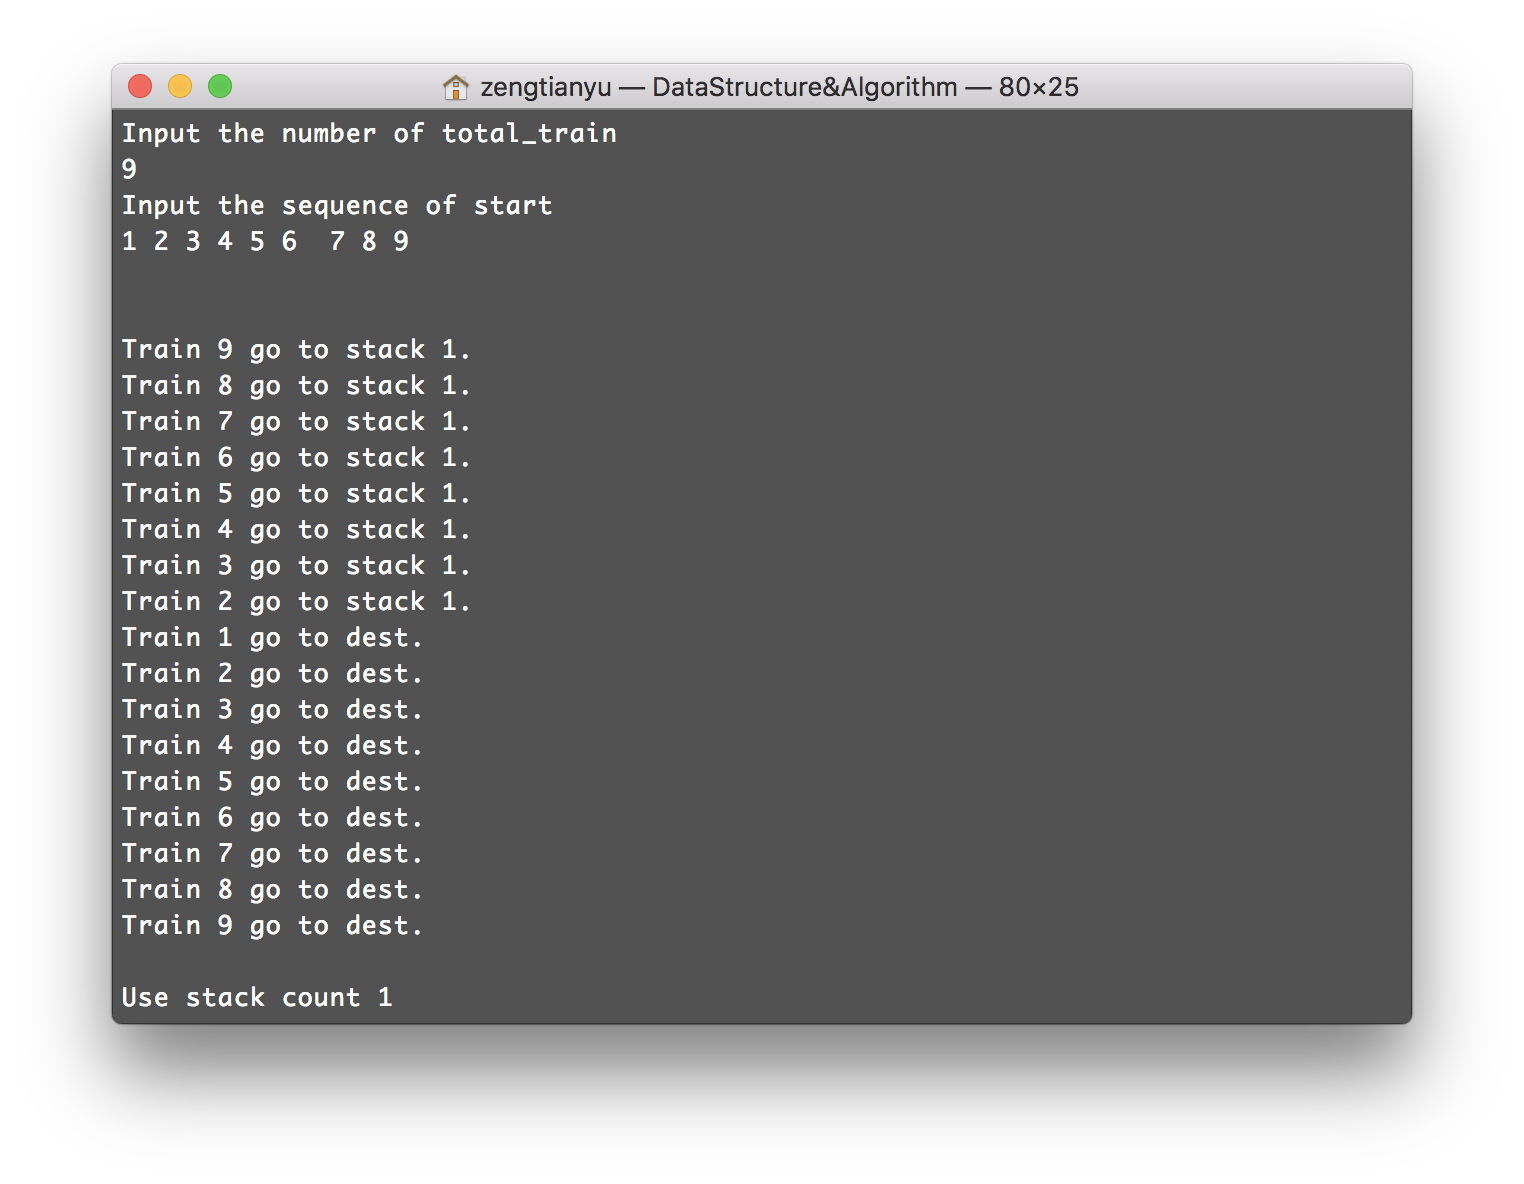
\includegraphics[width = 220pt]{Pics/pic7}}\\
\end{tabular}
\end{figure}

分析:从上面四组的运行结果来看,这两个方法在栈的使用上面是几乎一样的,在使用栈的个数上面是一致的,这一定程度上能够互相验证算法的正确性。与互联网上的相关算法相比,我们的两个算法在结果上面保持一致。因此,我们的两个方法是准确的。

\section{分工、贡献与自我评分}

\begin{table}[H]
	\centering
\begin{tabular}{|c|c|c|c|}
\hline
	& 分工 & 贡献度 & 自我评分\\
\hline
	曾天宇 & 讨论方法一、实现方法二、文档书写和编译$\LaTeX$ & 0.33 & 10/10\\
	陈鸿峥 & 讨论和实现方法一、$\LaTeX$模版书写 & 0.33 & 10/10\\
	黄杨峻 & 讨论和实现方法一、文档书写 & 0.33 & 10/10\\
\hline
\end{tabular}
\end{table}

\section{项目总结}
% (收获、体会,若实验课上未完成调试,要认真找出错误并分析原因等。)
做这个项目一开始也是遇到了点困难,审题上出现点失误(误认为车厢可以在缓冲轨道间单向移动)导致模型有误,浪费了很多时间。但重新审题后,我们很快就找到了正确的模型,并且快速实现了代码的编写。这次项目虽然简单,只涉及到栈的简单性质,但因为本次实验是我们第一次小组合作,所以在沟通协作方面可能做的还是有点不足,效率不够高,还有提升的空间。下次实验之前应提前做好分工,将工作完成得更好。


\section{程序清单}

\subsection{方法一}

\begin{lstlisting}
#include <iostream>
#include <stack>
#include <vector>
using namespace std;

int main()
{
 // read in sequence
 cout << "Welcome to the rearrangement system of train cabins"<<endl;
 cout << "Input the number of the cabins and the sequence of them."<<endl;
 int n,step=0;
 vector<int> trainLst;
 cin >> n;
 for (int i = 0; i < n; ++i)
 {
  int num;
  cin >> num;
  //trainLst.push_back(num);
        trainLst.insert(trainLst.begin(),num);
 }
 vector<  stack<int>  > station;

 // rearrangement
 int now = 0;
 for (auto train : trainLst)
 {
  // directly move out the train satisfies the order
  if (train == now + 1)
  {
   cout << "Train " << train << " move out" << endl;
   step++;
   now++;
   while (true)
   {
    bool flag_in = false;
    for (auto psrcst = station.begin(); psrcst < station.end(); ++psrcst)
     while (!psrcst->empty() && psrcst->top() == now + 1)
     {
      cout << "Train " << psrcst->top() << " move out from stack " << (psrcst-station.begin()) << endl;
      step++;
      psrcst->pop();
      now++;
      flag_in = true;
     }
    if (flag_in)
     continue;
    else
     break;
   }
   continue;
  }

  // push the current train into the previous stack
  int cnt = 0;
  bool flag = false;
  for (auto ptmpst = station.begin(); ptmpst < station.end(); ++ptmpst)
   if ((!ptmpst->empty() && train < ptmpst->top()) || ptmpst->empty())
   {
    ptmpst->push(train);
    cout << "Train " << train << " push into stack " << cnt << endl;
    step++;
    flag = true;
    break;
   }
   else
    cnt++;
  if (!flag)
  {
   stack<int> tmpst;
   tmpst.push(train);
   cout << "Train " << train << " push into stack " << cnt << endl;
   step++;
   station.push_back(tmpst);
  }
 }
 cout << "Total stacks used: " << station.size() << endl;
 cout << "Total steps used: " << step <<endl;
 return 0;
}
\end{lstlisting}

\subsection{方法二}
\begin{lstlisting}
#include <iostream>
#include <stack>
#include <vector>
#include<cstdlib>
using namespace std;

vector<stack<int>> stk;
int outmin = 1;

void goTo(int temp, bool dest, int num){
    if (dest) {
        cout<<"Train "<<temp<<" go to dest. "<<endl;
        outmin += 1;
    }else{
        cout<<"Train "<<temp<<" go to stack "<<num+1<<". "<<endl;
    }
}

void moveToStack(int temp, bool createNew){
    int index = 0;
    int min = 999999;
    if (createNew) {
        bool flag1 = false, flag2 = false;
        for (int i = 0; i<stk.size(); i++) {
            if (stk.at(i).empty()) {
                index = i;
                flag1 = true;
            }
            else if (stk.at(i).top()>temp) {
                if (min<stk.at(i).top()) {
                    //todo
                }else{
                    min = stk.at(i).top();
                    index = i;
                    flag2 = true;
                }
            }
        }
        if (flag1&&!flag2) {
            stk.at(index).push(temp);
        }else if (flag2){
            stk.at(index).push(temp);
        }
        else{
            stack<int> sk;
            sk.push(temp);
            stk.push_back(sk);
            index = (int)stk.size()-1;
        }
    }else{
        
        index = 0;
        for (int i = 0; i<stk.size(); i++) {
            if (stk.at(i).top()>temp) {
                if (min<stk.at(i).top()) {
                    //todo
                }else{
                    min = stk.at(i).top();
                    index = i;
                }
            }
        }
        stk.at(index).push(temp);
    }
    goTo(temp, false, index);
    //cout<<stk.size()<<endl;
}

int main(){
    int count;
    cout<<"Input the number of total_train"<<endl;
    cin>>count;
    int series[count], delta[count];
    cout<<"Input the sequence of start "<<endl;
    for (int i = 0; i<count; i++) {
        cin>>series[count-1-i];
    }
    cout<<endl;
    for (int i = 0; i<count-1; i++) {
        delta[i] = series[i+1]-series[i];
    }
    cout<<endl;
    for (int i = 0; i<count; i++) {
        for (int k = 0; k<stk.size(); k++) {
            if (stk.at(k).empty()) {
                continue;
            }
            if (stk.at(k).top()==outmin) {
                goTo(stk.at(k).top(), true, 0);
                stk.at(k).pop();
                if (!stk.at(k).empty()) {
                    k--;
                }
            }
        }
        if(series[i] == 1 || series[i] == outmin){
            //go to dest.
            goTo(series[i], true, 0);
            continue;
        }
        if (delta[i-1]<0) {
            moveToStack(series[i], i==0);
        }else{
            moveToStack(series[i], true);
        }
        for (int k = 0; k<stk.size(); k++) {
            if (stk.at(k).empty()) {
                stk.erase(stk.begin()+k);
            }
        }
        //cout<<"**"<<outmin<<"**\n";
    }
    for (int i = outmin; i<=count; i++) {
        for (int k = 0; k<stk.size(); k++) {
            if (stk.at(k).empty()) {
                continue;
            }
            if (stk.at(k).top() == i) {
                goTo(stk.at(k).top(), true, 0);
                stk.at(k).pop();
                break;
            }
        }
    }
    cout<<endl<<"Use stack count "<<stk.size()<<endl;
    return 0;
}


\end{lstlisting}


\end{document}